\documentclass[11pt,a4paper]{article}
\usepackage{graphicx}
\usepackage{amsmath}
\usepackage{amssymb}
\usepackage{multicol}
\usepackage{tcolorbox}
\usepackage{xcolor}
\usepackage{geometry}
\usepackage{tikz}
\geometry{margin=1in}

% Define colors
\definecolor{mlblue}{RGB}{31, 119, 180}
\definecolor{mlorange}{RGB}{255, 127, 14}
\definecolor{mlgreen}{RGB}{44, 160, 44}
\definecolor{mlred}{RGB}{214, 39, 40}
\definecolor{mlpurple}{RGB}{148, 103, 189}

\title{\Large\textbf{Discovery Learning: K-Means Step-by-Step}\\
\vspace{0.5em}
\large Understanding the K-Means Algorithm Through Practice}
\author{Machine Learning for Smarter Innovation - Week 1}
\date{}

\begin{document}
\maketitle

\section*{Learning Objectives}
By completing this exercise, you will:
\begin{itemize}
    \item Understand each step of the K-means algorithm
    \item Practice manual clustering to build intuition
    \item See how computers optimize cluster assignments
    \item Learn to predict convergence patterns
\end{itemize}

\section*{The K-Means Algorithm}
\begin{tcolorbox}[colback=mlblue!10, colframe=mlblue!50, title=Algorithm Steps]
\begin{enumerate}
    \item \textbf{Initialize}: Choose k initial cluster centers (randomly or using k-means++)
    \item \textbf{Assign}: Assign each point to the nearest cluster center
    \item \textbf{Update}: Move centers to the mean of their assigned points
    \item \textbf{Repeat}: Continue until centers stop moving (convergence)
\end{enumerate}
\end{tcolorbox}

\section*{Exercise 1: Manual K-Means (k=2)}
Given these 10 innovation projects with their complexity (x) and impact (y) scores:

\begin{center}
\begin{tabular}{|c|c|c|c|c|c|c|c|c|c|c|}
\hline
\textbf{Project} & A & B & C & D & E & F & G & H & I & J \\
\hline
\textbf{Complexity (x)} & 2 & 3 & 8 & 9 & 2 & 3 & 8 & 9 & 5 & 5 \\
\hline
\textbf{Impact (y)} & 2 & 3 & 8 & 9 & 8 & 9 & 2 & 3 & 5 & 6 \\
\hline
\textbf{Your Cluster} & & & & & & & & & & \\
\hline
\end{tabular}
\end{center}

\subsection*{Step 1: Initialize Centers}
Let's start with centers at Project A (2,2) and Project C (8,8).

\begin{tcolorbox}[colback=mlorange!10, colframe=mlorange!50, title=Your Work]
Calculate distances from each point to both centers using: $d = \sqrt{(x_2-x_1)^2 + (y_2-y_1)^2}$

\begin{multicols}{2}
\textbf{Distance to Center 1 (2,2):}
\begin{itemize}
    \item A to C1: \underline{\hspace{2cm}}
    \item B to C1: \underline{\hspace{2cm}}
    \item C to C1: \underline{\hspace{2cm}}
    \item D to C1: \underline{\hspace{2cm}}
    \item E to C1: \underline{\hspace{2cm}}
\end{itemize}

\textbf{Distance to Center 2 (8,8):}
\begin{itemize}
    \item A to C2: \underline{\hspace{2cm}}
    \item B to C2: \underline{\hspace{2cm}}
    \item C to C2: \underline{\hspace{2cm}}
    \item D to C2: \underline{\hspace{2cm}}
    \item E to C2: \underline{\hspace{2cm}}
\end{itemize}
\end{multicols}
\end{tcolorbox}

\subsection*{Step 2: First Assignment}
Assign each project to its nearest center:

\begin{tcolorbox}[colback=mlgreen!10, colframe=mlgreen!50, title=Cluster Assignment]
\textbf{Cluster 1 members}: \underline{\hspace{8cm}}\\
\textbf{Cluster 2 members}: \underline{\hspace{8cm}}
\end{tcolorbox}

\subsection*{Step 3: Update Centers}
Calculate new center positions (mean of assigned points):

\begin{tcolorbox}[colback=mlpurple!10, colframe=mlpurple!50, title=New Centers]
\textbf{New Center 1}:\\
x = (sum of x-coordinates) / (number of points) = \underline{\hspace{3cm}}\\
y = (sum of y-coordinates) / (number of points) = \underline{\hspace{3cm}}\\

\textbf{New Center 2}:\\
x = \underline{\hspace{3cm}}\\
y = \underline{\hspace{3cm}}
\end{tcolorbox}

\section*{Exercise 2: Predicting Convergence}
\begin{multicols}{2}
\textbf{Draw your predictions:}\\
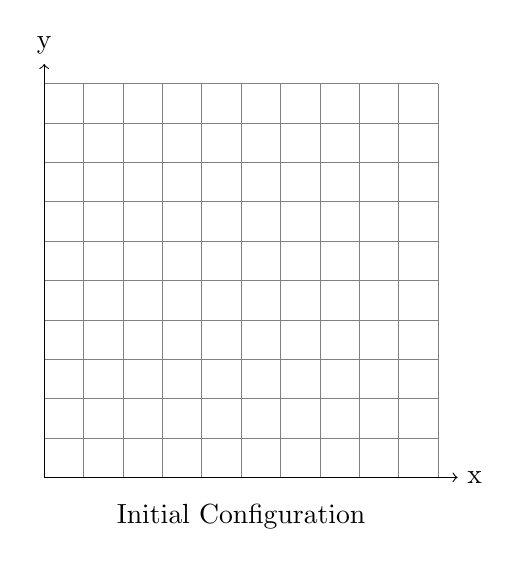
\begin{tikzpicture}[scale=0.5]
    \draw[step=1cm,gray,very thin] (0,0) grid (10,10);
    \draw[->] (0,0) -- (10.5,0) node[right] {x};
    \draw[->] (0,0) -- (0,10.5) node[above] {y};
    \node at (5,-1) {Initial Configuration};
\end{tikzpicture}

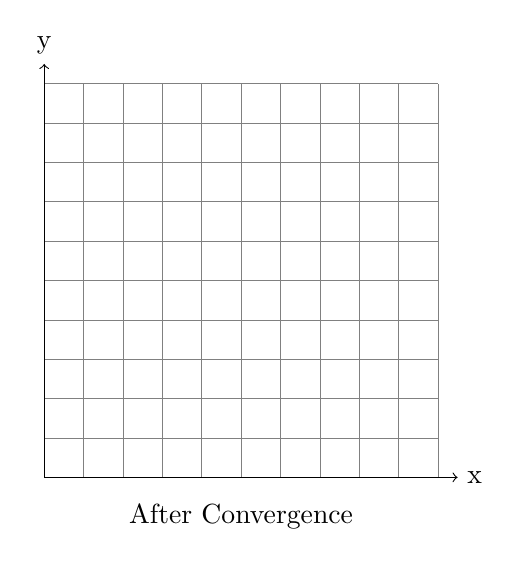
\begin{tikzpicture}[scale=0.5]
    \draw[step=1cm,gray,very thin] (0,0) grid (10,10);
    \draw[->] (0,0) -- (10.5,0) node[right] {x};
    \draw[->] (0,0) -- (0,10.5) node[above] {y};
    \node at (5,-1) {After Convergence};
\end{tikzpicture}
\end{multicols}

\section*{Exercise 3: Algorithm Behavior}
Answer these questions based on your manual calculation:

\begin{enumerate}
    \item How many iterations did it take to converge? \underline{\hspace{3cm}}
    \item What would happen with different initial centers? \underline{\hspace{5cm}}
    \item Which points might switch clusters if k=3? \underline{\hspace{5cm}}
    \item What's the total within-cluster sum of squares? \underline{\hspace{4cm}}
\end{enumerate}

\section*{Exercise 4: Real Implementation}
Compare your manual results with sklearn's implementation:

\begin{tcolorbox}[colback=gray!10, colframe=gray!50, title=Python Code]
\begin{verbatim}
from sklearn.cluster import KMeans
import numpy as np

# Your data
X = np.array([[2,2], [3,3], [8,8], [9,9], [2,8], 
              [3,9], [8,2], [9,3], [5,5], [5,6]])

# Run K-means
kmeans = KMeans(n_clusters=2, random_state=42)
labels = kmeans.fit_predict(X)
centers = kmeans.cluster_centers_

print("Cluster assignments:", labels)
print("Final centers:", centers)
print("Iterations:", kmeans.n_iter_)
\end{verbatim}
\end{tcolorbox}

\textbf{Your observations}:
\begin{itemize}
    \item Did sklearn get the same clusters? \underline{\hspace{5cm}}
    \item Were the final centers identical? \underline{\hspace{5cm}}
    \item Why might there be differences? \underline{\hspace{6cm}}
\end{itemize}

\section*{Key Insights}
\begin{itemize}
    \item K-means is \textbf{deterministic} given the same initial centers
    \item Different initializations can lead to \textbf{different final clusters}
    \item The algorithm finds a \textbf{local optimum}, not necessarily global
    \item Convergence typically happens in \textbf{5-10 iterations}
    \item The result minimizes \textbf{within-cluster variance}
\end{itemize}

\section*{Challenge Extensions}
\begin{enumerate}
    \item Try k=3 with the same data. How do clusters change?
    \item Add an outlier at (15, 15). What happens to the clusters?
    \item Calculate the silhouette score for k=2 vs k=3
    \item Implement one iteration in Python without using sklearn
\end{enumerate}

\section*{Reflection Questions}
\begin{tcolorbox}[colback=mlred!10, colframe=mlred!50, title=Think Deeper]
\begin{enumerate}
    \item When would you choose a different k value in real applications?
    \item How could you automate the choice of initial centers?
    \item What business decisions could you make from these clusters?
    \item How would you validate that your clusters are meaningful?
\end{enumerate}
\end{tcolorbox}

\end{document}